\documentclass[8pt]{beamer}
\mode<presentation> {
\usetheme{Madrid}
\usecolortheme{crane}
}
\usepackage{graphicx}
\usepackage{subfig}
\usepackage{booktabs} % permite usar  \toprule, \midrule y \bottomrule en tablas
\usepackage{listings} % permite citar codigo a partir de un archivo externo a este documento
\lstset{frame=single, language=bash, basicstyle=\small} % Setea listings para encerrar el codigo en u marco y definir el lenguaje y el tamaño del codigo
\usepackage{ragged2e} % paquete que permite justificar texto en la clase beamer
\justifying
%----------------------------------------------------------------------------------------
%	PAGINA DE TITULO
%----------------------------------------------------------------------------------------

\title[Man Git]{Manual de uso Git}
\author{Samuel Pavon}
\institute[UCV-Libre]
{
Comunidad de conocimiento Libre de la Universidad Central de Venezuela \\
\medskip
\textit{contacto@ucvlibre.org.ve}
}
\date{2016}

\begin{document}

\begin{frame}
\fontsize{12}{8}\selectfont
\titlepage
\end{frame}

\begin{frame}
\frametitle{Contenido}
\tableofcontents 
\end{frame}

%----------------------------------------------------------------------------------------
%	LAMINAS DE LA PRESENTACION
%----------------------------------------------------------------------------------------

%------------------------------------------------
\section{Introducci\'on} % Sections can be created in order to organize your presentation into discrete blocks, all sections and subsections are automatically printed in the table of contents as an overview of the talk
%------------------------------------------------
\subsection{}
\begin{frame}
\frametitle{introducci\'on}
Este manual pretende ser una gu\'ia completa del sistema de control de versiones Git 
\end{frame}
%------------------------------------------------
\section{Configurando Repositorio} 
%------------------------------------------------
\subsection{Git Init} 
\begin{frame}
\frametitle{Configurando Repositorio}
\textbf{Git Init}\\
El comando \texttt{git init} crea un nuevo repositorio Git. Puede ser usado para convertir un proyecto sin control de versi\'on en un repositorio Git o iniciar un nuevo repositorio vacio. La gran mayor\'ia de los comandos de Git no est\'an disponibles fuera de un repositorio inicializado, por consiguiente, usualmente este es el primer comando que se tendra que correr en un proyecto nuevo.\\
Al ejecutar \texttt{git init} se crea autom\'aticamente un sub-directorio de nombre \texttt{.git} en el directorio raiz del proyecto, el cual contiene toda la metadata necesaria para el repo. Aparte del directorio \texttt{.git}, el resto de un proyecto existente se mantiene inalterado.\\
\medskip
\textbf{Uso:}\\
\lstinputlisting[firstline=2,lastline=2]{mangit.sh}
Este comando transforma el directorio en donde se este ubicado en un repositorio Git. Esto añade la carpeta \texttt{.git} al directorio en donde estemos ubicados y hace posible empezar a utilizar el registro de versiones del proyecto
\lstinputlisting[firstline=3, lastline=3]{mangit.sh}
Crea un Repositorio Git vacio en el directorio especificado. Este comando creara un nuego directorio llamado \texttt{directory} cuyo contenido solo sera el subdirectorio \texttt{.git}
\end{frame}
\begin{frame}
\frametitle{Configurando Repositorio}

\lstinputlisting[firstline=4, lastline=4]{mangit.sh}
Crea un repositorio Git vacio, pero omitiendo el directorio de trabajo. Repositorios compartidos siempre deben ser creados con el par\'ametro \texttt{--bare} (ver discusi\'on mas abajo). A modo de convenci\'on, los repositorios que se arrancan con el par\'ametro \texttt{--bare} suelen terminar en \texttt{.git}. Por ejemplo, la versi\'on bare de un repositorio llamado \texttt{mi-proyecto} deberia ser guardada en un directorio llamado \texttt{mi-proyecto.git}\\
\medskip
\textbf{Discusi\'on}\\
El comando \texttt{git init} es una forma increiblemente f\'acil de crear un nuevo proyecto con control de versi\'on. Git no requiere que se cree un repositorio, se importan archivos y verificar copias funcionales como si sucede con otros sistemas de control de versiones. En Git todo lo que se necesista hacer es ubicarse en la carpeta de un proyecto y correr \texttt{git init} y se tendr\'a un repositorio Git totalmente funcional. Sin embargo para la mayor\'ia de los proyectos, \texttt{git init} solo necesita ser ejecutado una sola vez para crear un repositorio central; los desarrolladores generalmente no usan \texttt{git init} para crear sus repositorios locales. En lugar de esto, usualmente usan \texttt{git clone} para copiar un repositorio existente en sus m\'aquinas locales.  

\end{frame}


\begin{frame}
\frametitle{Configurando Repositorio}
\textbf{Repositorios Bare}\\
\medskip
El par\'ametro \texttt{--bare} crea un repositorio que no cuenta con un directorio de trabajo, haciendo imposible editar archivos y hacer cambios commit en esos repositorios. Repositorios centrales deben siempre ser creado como repositorios bare ya que hacer push de branches a repositorios non-bare tiene el potencial de sobrescribir cambios. Pensemos en \texttt{--bare} como una manera de marcar un repositorio como un almac\'en, en oposici\'on a un entorno de desarrollo. Esto significa que para virtualmente todos los flujos de trabajo de Git, el repositorio central es bare, y los repositorios locales de desarrollo son non-bare.\\
\medskip
\begin{figure}[h]
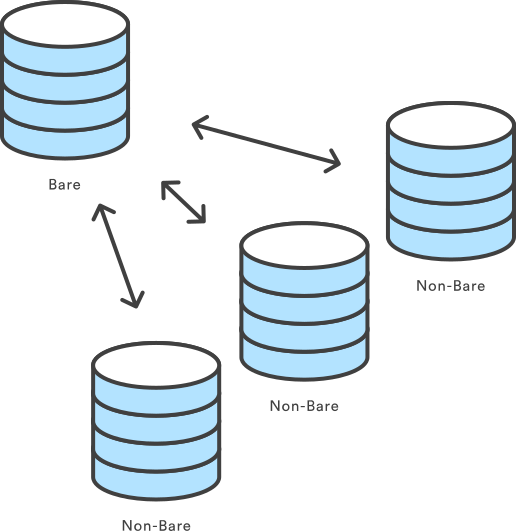
\includegraphics[scale=0.35]{imagenes/01.png}
\centering
\end{figure}
\end{frame}

%------------------------------------------------
\begin{frame}
\frametitle{Configurando Repositorio}
\textbf{Ejemplo}\\
Desde que \texttt{git clone} es la manera mas conveniente de crear una copia local de un proyecto, el uso mas com\'un para \texttt{git init} es crear un repositorio central:
\lstinputlisting[firstline=6, lastline=8]{mangit.sh}
En este ejemplo primero se hace loguin v\'ia SSH en el servidor que contendr\'a el repositorio central, luego se navega hasta el directorio donde estar\'a guardado el proyecto y finalmente se usa el par\'ametro \texttt{--bare} para crear el repositorio central de almac\'en. Los desarrolladores entonces tendr\'an que usar el comando \texttt{git clone} para crear una copia del repositorio en sus maquinas de desarrollo.
\end{frame}

%------------------------------------------------
\subsection{git clone}

\begin{frame}
\frametitle{Configurando Repositorio}
\textbf{git clone}\\
\medskip
el comando \texttt{git clone} copia un repositorio Git existente. La copia de trabajo es un repositorio Git completamente establecido; es decir, tiene su propio historial, maneja sus propios archivos y cuenta con un entorno completamente aislado del repositorio original.
Como conveniencia, el clonado crea autom\'aticamente una conexi\'on remota con el repositorio original, esto hace que sea muy f\'acil interactuar con el repositorio central\\
\medskip
\textbf{uso}\\
\medskip
\lstinputlisting[firstline=10, lastline=10]{mangit.sh}
Esto clona un repositorio ubicado en \texttt{<repo>} en la m\'aquina local. El repositorio original puede ser ubicado en el sistema de archivos local o en una maquina remota via HTTP o SSH.
\lstinputlisting[firstline=11, lastline=11]{mangit.sh}
Clona un repositorio ubicado en \texttt{<repo>} en un directorio llamado \texttt{<directory>} en la m\'aquina local.\\
\medskip
\textbf{Discusi\'on}\\
\medskip
Si un proyecto ha sido configurado como repositorio central, el comando \texttt{git clone} es la forma mas com\'un para los usuarios de obtener una copia de desarrollo. Como \texttt{git init},  clonar es generalmente una operaci\'on que se realiza una sola vez, cuando un desarrollador ha obtenido una copia funcional, toda la operaci\'on de control de versi\'on y colaboraciones son manejadas a trav\'es del repositorio local.
\end{frame}
%------------------------------------------------

\begin{frame}
\frametitle{Configurando Repositorio}
\textbf{Colaboraci\'on Repo-To-Repo}\\
\medskip
Es importante entender que la l\'ogica de Git con respecto al concepto de "copia funcional" es muy diferente a las copias funcionales que se tienen cuando se trabaja con un repositorio de tipo SVN. A diferencia de SVN, Git no hace distinci\'on entre una copia funcional y el repositorio central; todos los repositorios que se crean con 
Git son totalmente establecidos.
Esto hace que la colabroraci\'on con Git sea fundamentalmente diferente que con SVN. Mientras SVN depende de la relaci\'on entre el repositorio central y la copia funcional, el modelo de colaboraci\'on de Git esta basado en un modelo de interacci\'on repositorio-a-repositorio. En lugar de revisar una copia funcional en un repositorio central SVN, se puede hacer push o pull commits de un repositorio a otro. 
\begin{figure}
  \centering
  \subfloat{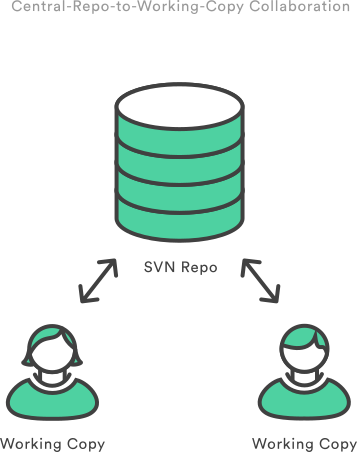
\includegraphics[scale=0.3]{imagenes/03.png}}\qquad \qquad
  \subfloat{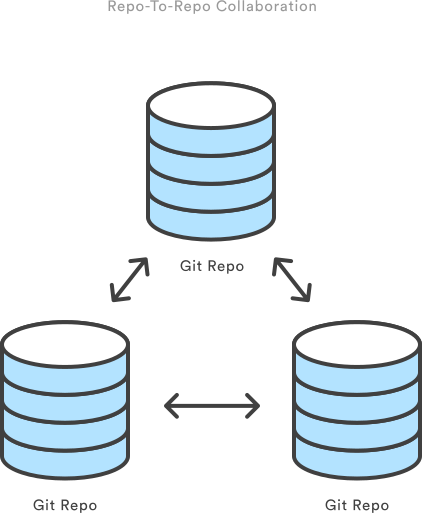
\includegraphics[scale=0.3]{imagenes/02.png}}
\end{figure}

\end{frame}

%------------------------------------------------

\begin{frame}
\frametitle{Configurando Repositorio}
Sin embargo no hay nada que nos detenga para dar un significado especial a ciertos repositorios. Por ejemplo, simplemente designando un repositorio Git como "Central" es posible replicar un flujo de trabajo centralizado usando Git. El punto se centra es que llevemos nuestros proyectos mas por convenciones que por ataduras que nos imponga el sistema de control de versi\'on.\\
\medskip
\textbf{Ejemplo}\\
\medskip
El siguiente ejemplo demuestra como obtener una copia local de un repositorio central alojado en un servidor accesible en el dominio \texttt{example.com} usando el nombre de usuario SSH \texttt{john}:
\lstinputlisting[firstline=13, lastline=15]{mangit.sh}

el primer comando inicia un nuevo repositorio Git en el directorio \texttt{my-project} de una maquina local y propaga todo el contenido del repositorio central en \'el. Ahora (estando ubicado en el repositorio local) se puede comenzar a editar archivos, hacer commits e interactuar con otros repositorios. Se puede notar ademas que la extensi\'on \texttt{.git} del directorio es omitida en el repositorio clonado; esto refleja el status de non-bare de la copia local.
\end{frame}

%------------------------------------------------
\subsection{git config}
\begin{frame} 
\frametitle{Configurando Repositorio}
\textbf{git config}\\
\medskip
el comando \texttt{git config} permite configurar la instalaci\'on de Git (o un repositorio individual) desde la l\'inea de comandos. Este comando puede definir cualquier cosa desde las preferencias de usuario hasta el comportamiento de un repositorio. Gran parte de las opciones de configuraci\'on son listadas a continuaci\'on.\\
\medskip
\textbf{Uso}\\
\medskip
\lstinputlisting[firstline=17, lastline=17]{mangit.sh}
Define el nombre del autor a ser usado para todos los commits en el repositorio que se este usando actualmente. Tipicamente se querr\'a usar el par\'ametro \texttt{--global} para fijar las opciones de configuraci\'on para el usuario actual.
\lstinputlisting[firstline=18, lastline=18]{mangit.sh}
Define el nombre de autor a ser usado para todos los commits por el usuario actual.
\lstinputlisting[firstline=19, lastline=19]{mangit.sh}
Define el email del autor a ser usado por todos los commits hechos por el usuario actual.
\lstinputlisting[firstline=20, lastline=20]{mangit.sh}
Crea un atajo para un comando Git
\end{frame}

%------------------------------------------------

\begin{frame}
\frametitle{Configurando Repositorio}
\lstinputlisting[firstline=21, lastline=21]{mangit.sh}
Define el editor de texto usado por los comandos para todos los usuarios en la maquina local. El argumento <editor> debe ser el comando que ejecuta el editor deseado (ejemplo: vi) 
\lstinputlisting[firstline=22, lastline=22]{mangit.sh}
Abre el archivo de configuracion global en un editor de texto para una edici\'on manual.
\textbf{Discusi\'on}\\
\medskip
Todas las opciones d configuraci\'on est\'an guardadas en archivos de texto plano, asi que el comando \texttt{git config} es una interface de linea de comando realmente conveniente. Generalmente solo se necesitara configurar la instalaci\'on la primera vez que se comience a trabajar en una nueva maquina donde se quiera desarrollar, y para virtualmente todos los casos sera mas conveniente usar el par\'ametro \texttt{--global}. Git guarda las opciones de configura\'on en tres archivos separados, lo que permite definir opciones para repositorios, usuarios o todo el sistema:\\
\begin{itemize}
\item \texttt{<repo>/.git/config – Repository-specific settings.}
\item \texttt{~/.gitconfig – User-specific settings. This is where options set with the --global flag are stored.} 
\item \texttt{\$(prefix)/etc/gitconfig – System-wide settings.} 
\end{itemize}
cuando las opciones en estos archivos entran en conflicto, las configuraciones locales sobrescriben las configuraciones de usuarios, que a su vez sobrescriben las del sistema
\end{frame}

%------------------------------------------------

\begin{frame}
\frametitle{Configurando Repositorio}
si se abre alguno de los archivos mencionados anteriormente se observar\'a algo como lo
siguiente:
\lstinputlisting[firstline=24, lastline=34]{mangit.sh}
Se puede editar manualmente estos valores y se obtendr\'a exactamente el mismo efecto que al usar el comando \texttt{git config}\\
\medskip
\textbf{Ejemplo}\\
\medskip
La primera cosa que se querr\'a hacer luego de instalar Git es definir un nombre/email y personalizar algunos de las configuraciones por defecto. Una confiuguraci\'on inicial t\'ipica luce algo parecido a lo siguiente:
\lstinputlisting[firstline=36, lastline=38]{mangit.sh}
\lstinputlisting[firstline=39, lastline=40]{mangit.sh}

\end{frame}

%------------------------------------------------

\begin{frame}
\frametitle{Configurando Repositorio}
\lstinputlisting[firstline=41, lastline=45]{mangit.sh}
Estos comandos producir\'an el archivo \texttt{\~/.gitconfig} que mostramos como ejemplo anteriormente
\end{frame}

%------------------------------------------------
\section{Guardando cambios}
\subsection{git add}
\begin{frame}
\frametitle{Guardando Cambios}
\textbf{git add}\\
\medskip
El comando \texttt{git add} agrega un cambio realizado en el directorio de trabajo a la "staging area" de Git. Le avisa a Git que se quiere incluir actualizaciones a un archivo particular en el siguiente commit. sin embargo, \texttt{git add} realmente no afecta el repositorio de una manera significativa (los cambios no son realmente hechos hasta que no se corra \texttt{git commit}.En conjunci\'on con estos comandos, tambi\'en se necesitar\'a \texttt{git status} para ver el estado del directorio de trabajo y de la "staging area".\\
\medskip
\textbf{Uso}
\lstinputlisting[firstline=49, lastline=49]{mangit.sh}
Agrega todos los cambios en \texttt{<file>} para el siguiente commit.
\lstinputlisting[firstline=50, lastline=50]{mangit.sh}
  Agrega todos los cambios en \texttt{<directory>} para el siguiente commit
\lstinputlisting[firstline=51, lastline=51]{mangit.sh}
Inicia una sesi\'on interactiva de "staging" que permite escoger porciones de archivos para agregar a un pr\'oximo commit. Esto presentar\'a una porci\'on de cambios y esperara por un comando. Para confirmar los cambios se confirma con \texttt{y}, \texttt{n} para ignorar el pedazo, \texttt{s} para dividir en pedazos mas pequeños, \texttt{e} para editar manualmente el pedazo y \texttt{q} para salir.
\end{frame}

%------------------------------------------------

\begin{frame}
\frametitle{Guardando Cambios}
\textbf{Discusi\'on}\\
\medskip
Los comandos \texttt{git add} y \texttt{git commit} componen el flujo de trabajo fundamental de Git. Son los dos comandos que todo usuario Git necesita entender, sea cual sea el modelo de colaboraci\'on que se este usando. Estos comandos son los que dan significado a registro de versiones de un proyecto en el historial de un repositorio. El desarrollo de un proyecto gira entorno al patr\'on b\'asico de editar/agregar cambios a la staging area/commit. Primero se edita cualquier archivo en el directorio de trabajo; cuando se esta listo para guardar una copia del estado actual del proyecto, se pasan los cambios al staging area con \texttt{git add}; cuando se esta conforme con los cambios de la staging area se hace commit al historial del proyecto con \texttt{git commit}.\\
\medskip
\begin{figure}
  \centering
  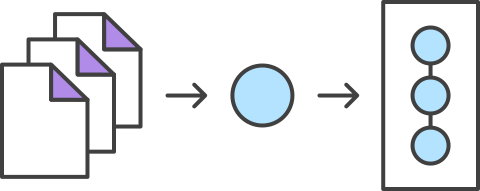
\includegraphics[scale=0.4]{imagenes/04.png}
\end{figure}

\end{frame}

%------------------------------------------------

\begin{frame}
\frametitle{Guardando cambios}
Cabe destacar que el comando \texttt{git add} necesita ser invocado cada vez que se altere un arhcivo por mas m\'inimo que sea el cambio. Esto puede parecer redundante, pero es este flujo de trabajo permite que sea mucho mas sencillo mantener un proyecto organizado.\\
\medskip
\textbf{La Staging Area}\\
\medskip
La "Staging Area" es una de las caracter\'isticas \'unicas de Git y puede ser un poco dificil de entender al principio si se viene de utilizar otros sistemas de registro de versiones como SVN o Mercurial. Ayuda a entender el pensar en el "staging Area" como un buffer entre el directorio de trabajo y el historial del proyecto. En lugar de hacer commit de todos los cambios que se hacen despu\'es del \'ultimo commit, el "stage" permite agrupar cambios relacionados en unas instant\'anes altamente focalizadas antes de hacer el commit al historial del proyecto. Esto implica que se puede hacer todo tipo de ediciones a archivos que no est\'en relacionados entre si, luego ir un poco atr\'as y dividirlos en commit l\'ogicos a\~nadiendo cambios relacionados a la "staging Area"  y hacer commit de esos cambios pedazo a pedazo. Como en todo sistema de control de revisiones, es importante crear commits lo mas peque\~no posibles, de esta manera es mas f\'acil rastrear bugs y revertir cambios con un m\'inimo impacto en el resto del proyecto.\\
\medskip
\textbf{Ejemplo}\\
\medskip
Para crear un commit inicial en el directorio actual, se usa los dos comandos siguientes:
\lstinputlisting[firstline=53, lastline=54]{mangit.sh}

\end{frame}

%------------------------------------------------

\begin{frame}
\frametitle{Guardando Cambios}
Una vez que el proyecto este corriendo, nuevos archivos pueden ser a\`nadidos usando la ubicaci\'on con \textrm{git add}:
\lstinputlisting[firstline=55, lastline=56]{mangit.sh}
los comandos de arriba puede ser usados tambi\'en para registrar cambios en un archivo existente. Git no diferencia entre cambios "staging" en nuevos archivos Vs cambios en archivos que ya han sido agregados al repositorio.\\
\medskip
\subsection{git commit}
\textbf{git commit}\\
\medskip
El comando \texttt{git commit} envia una instant\'anea en el "staging area" hacia el historial del proyecto. Hacer commit de instant\'aneas puede ser pensando como versiones "seguras" de un proyecto; Git nunca las cambiar\'a a menos que sea pedido explicitamente. Ademas de \texttt{git add}, este es uno de los comandos mas importantes de Git. Cabe destacar que las instant\'aneas son consignadas al repositorio local y esto no requiere de ninguna interacci\'on con otros repositorios Git\\
\medskip
\textbf{Uso}\\
\lstinputlisting[firstline=58, lastline=58]{mangit.sh}
Consigna la instant\'anea que se encuentre en la "Staging Area". Esto lanzar\'a un editor de texto esperando a que se introduzca un mensaje commit. Luego de que se haya ingresado el mensaje, se salva el archivo y cierra el editor para crear el commit propiamente.
\end{frame}
\begin{frame}
\frametitle{Guardando Cambios}
\lstinputlisting[firstline=59, lastline=59]{mangit.sh}
Hacer commit de una instant\'anea, pero en lugar de lanzar el editor de texto usa \texttt{<message>} como mensaje commit.
\lstinputlisting[firstline=60, lastline=60]{mangit.sh}
Consignar una inst\'antanea de todos los cambios en el directorio de trabajo. Esto solo incluye modificaciones de los archivos rastreados (aquellos que han sido agregados con \texttt{git add} en alg\'un punto de su historial).\\
\medskip
\textbf{Discusi\'on}\\
\medskip
Las instant\'aneas siempre son consignadas al repositorio local. Git no te fuerza a interactuar con un repositorio central mientras no est\'es listo; tal como la "Staging Area" es un buffer entre el directorio de trabajo y el historial del proyecto, cada repositorio local de desarrollo es un buffer entre sus contribuciones y el repositorio central. Esto cambia el modelo b\'asico de desarrollo para los usuarios Git; en lugar de hacer cambios y hacer commit directamente en un repositorio central, los desarrolladores en Git tienen la oportunidad de acumular comiits en sus repositorios locales. Esto tiene much\'isimas ventajas sobre la colaboraci\'on con el estilo SVN: hace mas f\'acil dividir una caracter\'istica en commits at\'omicos, manteniendo commits relacionados agrupados en un conjunto, y teniendo un historial limpio antes de publicar a un repositorio central. Adem\'as le permite a los desarrolladores trabajar en entornos aislados, difiriendo alguna integraci\'on hasta que se este en un conveniente punto de quiebre. 

\end{frame}
%-----------------------------------------------------------
\begin{frame}
\frametitle{Guardando Cambios}
\textbf{Instant\'aneas, no diferencias}\\
\medskip
Apartando las distinciones pr\'acticas entre SVN y Git, sus implementaciones adem\'as siguen filosofias de dise\~n totalmente divergentes. Mientras que SVN rastrea \emph{diferencias} en un archivo, el control de versiones Git esta basado en \emph{instant\'aneas}. Por ejemplo, un commit en SVN consiste en un diff comparado con el archivo original a\~nadido al repositorio. Git, por otro lado, registra en \emph{contenido entero} de cada archivo en cada commit.
\begin{figure}
  \centering
  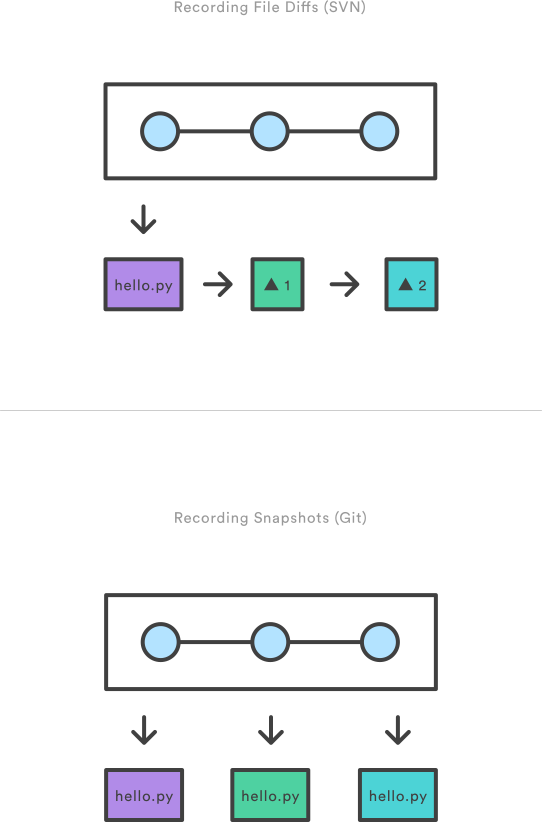
\includegraphics[scale=0.2]{imagenes/05.png}
\end{figure}
\end{frame}

%---------------------------------------------------------
\begin{frame}
\frametitle{Guardando Cambios}
Esto hace que muchas operaciones en Git sean mucho mas r\'apidas que en SVN, ya que una veri\'on particular no es "ensamblada" a partir de sus diffs; la revisi\'on completa de cada archivo esta disponible inmediatamente desde la base de datos interna de Git. El modelo de instant\'aneas de Git tiene un impacto importante en virtualmente cada aspecto del  modelo de control de versiones, afectando todo desde el branching y las herramientas de merging hasta los flujos de trabajo colaborativos.\\
\medskip
\textbf{Ejemplo}\\
\medskip
El siguiente ejemplo asume que se ha editado alg\'un contenido en un arhcivo llamado \texttt{hello.py} y esta listo para ser hecho commit al historial del proyecto. Primero, se necesita que el archivo sea enviado a la "staging Area" con \texttt{git add}, luego la instant\'anea puede ser consignado con \texttt{git commit}.
\lstinputlisting[firstline=62, lastline=63]{mangit.sh}
Lo anterior abrir\'a un editor de texto (personalizable via \texttt{git config} preguntando por un mensaje commit, ademas de una lista con lo que sera consignado:
\lstinputlisting[firstline=64, lastline=71]{mangit.sh}
\end{frame}

%----------------------------------------------------------
\begin{frame}
\frametitle{Guardando Cambios}
Git no requiere que los mensajes commit persigan ning\'un formato espec\'ifico, pero el formato can\'onico es resumir todo el commit en la primera linean en menos de 50 caracteres, dejar una l\'inea en blanco y luego dar una explicaci\'on detallada de que es lo que sea ha cambiado. Por ejemplo:
\lstinputlisting[firstline=72, lastline=75]{mangit.sh}
es de notar que muchos desarrolladores adem\'as gustan de usar el tiempo presente en sus mensajes de commit. Esto hace que se lea as como accciones en el repositorio, lo cual hace que muchas de las operaciones de rescritura del historial sean mas intuitivas.
\end{frame}
%---------------------------------------------------------
\section{Inspeccionando un Repositorio}
\subsection{git status}
\begin{frame}
\frametitle{Inspeccionado un Repositorio}
\textbf{git status}\\
\medskip
El comando \texttt{git status} muestra el estado de un directoriode trabajo y  de la "Staging Area". permite vver cuales cambios han sido puestos en la "Staging Area" cuales no, y cuales archivos no est\'an siendo rastreados por Git. La salida del status no muestra ninguna informaci\'on con respecto al historial del proyecto que ya sido consignado; para esto, se necesita usar \texttt{git log}.\\
\medskip
\textbf{Uso}\\
\medskip
\lstinputlisting[firstline=78, lastline=78]{mangit.sh}
Lista cuales archivos est\'an "staged", "unstaged", y "untracked".\\
\medskip
\textbf{Discusi\'on}\\
\medskip
El comando \texttt{git status} es un comando relativamente sencillo, simplemente muestra que es lo que ha estado sucediendo con \texttt{git add} y \texttt{git commit}. Los mensajes de status tambi\'en pueden incluir instrucciones relevantes para "staging/unstaging" archivos.  la siguiente salida de prueba muestra tres categor\'ias principales de \texttt{git status}:

\end{frame}

%---------------------------------------------------------
\begin{frame}
\frametitle{Inspeccionando un Repositorio}
\lstinputlisting[firstline=80, lastline=95]{mangit.sh}
\textbf{Ignorando archivos}\\
\medskip
Archivos sin rastrear t\'ipicamente caen en dos categori\'as; o son archivos que acaban de ser agregados al proyecto y no han sido consignados aun o son binarios compilados tipo archivos \texttt{.pyc, .obj, .exe}, etc. Mientras que agregar los primeros al la salida de \texttt{git status} es definitivamente beneficioso, incluir los segundos puede conducir a que sea haga dif\'icil que es lo que en realidad esta ocurriendo en un repositorio. Por esta raz\'on, Git permite ignorar archivos colocando las ubicaciones de los archivos a ignorar en un archivo especial llamado \texttt{.gitignore}. Todo archivo que se desee ignorar debe ser incluido en l\'inea aparte, y el simbolo * puede ser usado como comod\'in.
\end{frame}
\begin{frame}
\frametitle{Inspeccionado un Repositorio}
Por ejemplo agregando lo siguiente al archivo \texttt{.gitignore} de el directorio ra\'iz de un proyecto previene la aparici\'on de m\'odulos compilados de Python en \texttt{git status}:
\lstinputlisting[firstline=97, lastline=97]{mangit.sh}
\textbf{Ejemplo}\\
\medskip
Es una buena pr\'actica chequear el estado de un repositorio antes de consignar cambios, de esta manera no se consigna accidentalmente algo que en principio no se deseaba consignar. Este ejemplo muestra el status de l repositorio antes y despu\'es de "staging" y consignar una instant\'anea:
\lstinputlisting[firstline=99, lastline=107]{mangit.sh}
La salida del primer status mostrar\'a el archivo como "unstaged". La acci\'on \texttt{git add} se reflejar\'a en el segundo \texttt{git status} y la salida del status final dir\'a que no hay nada que consignar. Algunos comandos Git (ejemplo: \texttt{git merge)} requiere que el directorio de trabajo este limpio asi se evita la sobrescritura accidental de cambios.
\end{frame}

%--------------------------------------------------------------------------
\subsection{git log}
\begin{frame}
\frametitle{Inspeccionando un Repositorio}
\textbf{git log}\\
\medskip
el comando \texttt{git log} muestra las instant\'aneas que han sido consignadas; permite listar el historial del proyecto, filtrarlo y buscar por cambios espec\'ificos. Mientras \texttt{git status} permite inspeccionar el directorio de trabajo y la "Staging Area", \texttt{git log} solo opera con el historial de commits.\\
\medskip
\begin{figure}
  \centering
  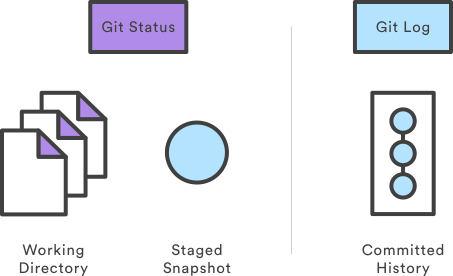
\includegraphics[scale=0.4]{imagenes/06.png}
\end{figure}
La salida de este comando puede ser personalizada de muchas maneras, desde un filtrado simple de commits hasta mostrarlos en un formato completamente definido por el usuario. Algunas de las mas comunes configuraciones de \texttt{git log} son presentadas a continuaci\'on.


\end{frame}

%---------------------------------------------------------
\begin{frame}
\frametitle{Inspeccionado un Repositorio}
\textbf{Uso}\\
\lstinputlisting[firstline=109, lastline=109]{mangit.sh}
Muestra el historial entero de commits usando el formato por defecto; si la salida toma mas de una pantalla, se puede usar la tecla \texttt{espacio} para moverse hacia abajo y \texttt{q} para salir.
\lstinputlisting[firstline=110, lastline=110]{mangit.sh}
Limita el n\'umero de commits al valor del argumento \texttt{<limit>}. Por ejemplo, \texttt{git log -n 3} mostrar\'a solo 3 commits.
\lstinputlisting[firstline=111, lastline=111]{mangit.sh}
condensa cada commit a una sola linea. Esto es \'util para tener un resumen de alto nivel del historial del proyecto.
\lstinputlisting[firstline=112, lastline=112]{mangit.sh}
Ademas de la informacii\'on ordinario de \texttt{git log}, incluye que archivos fueron alterados y el n\'umero relativo de l\'ineas que hans sido a\~nadidas o borradas para cada uno de ellos.
\lstinputlisting[firstline=113, lastline=113]{mangit.sh}
Muestra el parche representando cada commit. Esto muestra el diff complto de cada commit, la cual es la vista mas detallada que se puede obtener del historial de un proyecto.
\end{frame}

%--------------------------------------------------------
\begin{frame}
\frametitle{Inspeccionando un Repositorio}
\lstinputlisting[firstline=114, lastline=114]{mangit.sh}
Busca por commits de un autor particular. El argumento \texttt{<pattern>} puede ser una cadena sencilla o una expresi\'on regular.
\lstinputlisting[firstline=115, lastline=115]{mangit.sh}
Busca por commits con un mensaje de commit que corresponda con \texttt{<pattern>}, el cual puede ser una cadena sencilla o una expresi\'on regular.
\lstinputlisting[firstline=116, lastline=116]{mangit.sh}
Muestra solo los commits que ocurrieron entre \texttt{<since>} y \texttt{<until>}. Ambos argumentos tienen que ser o un commit ID, el nombre de un branch, HEAD, o cualquier otra clase de referencia de revisi\'on.
\lstinputlisting[firstline=117, lastline=117]{mangit.sh}
Solo muestra commits que incluyan el archivo especificado. Esta es una manera f\'acil de ver el historial de un archivo particular.
\lstinputlisting[firstline=118, lastline=118]{mangit.sh}
Algunas opciones \'utiles a considear. El par\'ametro \texttt{--graph} dibujar\'a un grafo basado en texto de los commits en el lado izquierdo de los mensajes commit \texttt{--decorate} agrega los nombres de los branches o las etiquetas de los commits que est\'an mostrados. \texttt{--oneline} muestra la informaci\'on del commit en una sola linea, logrando que sea mas f\'acil navegar a trav\'es de los commits a simple vista.
\end{frame}
\begin{frame}
\frametitle{Inspeccionado un Repositorio}
\textbf{Discusi\'on}\\
\medskip
El comando \texttt{git log} es una herramienta b\'asica de git para explorar el historial de un repositorio. Es lo que se usa cuando se necesita encontrar la versi\'on espec\'ifica de un proyecto o descifrar cuales cambios ser\'an introducidos al hacer un merging de un branch.
\lstinputlisting[firstline=120, lastline=121]{mangit.sh}
La mayor parte de esto es muy sencillo;sin embargo, la primera l\'inea necesita alguna explicaci\'on. La cadena de 40 caracteres luego de \texttt{commit} es un SHA-1 checksum del contenido del commit; esto sirve para dos prop\'ositos, el primero es asegurar la integridad del commit si alguna vez estuvo corrupto, el commit generar\'ia un checksum diferente; segundo, sirve como un identificador \'unico (ID) para el commit. Este ID puede ser usado en comandos como \texttt{git log <since>..<until>} para referirse a commits especi\'ificos. Por ejemplo, \texttt{git log 3157e..5ab91} mostrar\'a todo entre los commits con ID 3557e y 5ab91. Aparte de los checksum, nombres de branch (discutido en el m\'odulo Branch) y la palabra clave HEAD, existen otros m\'etodos comunes para referirse a commits individuales. HEAD siempre se refiere al commit actual, estando en un branch o un commit espec\'ifico.\\
El caracter \~~ es \'util para hacer referencias relativas de los padres de un commit. Por ejemplo, \texttt{3157\~~1} refiere al commit antes \texttt{3157e} y \texttt{HEAR\~~3} es el bisabuelo del commit actual.\\
La idea detr\'as de tosdos estos m\'etodos de indetificaci\'on es permitir realizar acciones basadas en commits espec\'ificos. El comando \texttt{git log} es generalmente el punto de inicio de estas interacciones, mientras permita encontrar los commits que se requieran para trabajar con ellos
\end{frame}
%--------------------------------------------------------

\begin{frame}
\frametitle{Inspeccionando un Repositorio}
\textbf{Ejemplo}\\
\medskip
Mas arriba en \texttt{uso} vimos varios ejemplos de \texttt{git log} pero muchas de esas opciones se pueden combinar en un solo comando:
\lstinputlisting[firstline=123, lastline=123]{mangit.sh}
Esto mostrar\'a un completo diff de todos los cambios que John Smith ha hecho en el archivo \texttt{hello.py}. La sintaxis ".." es una herramienta muy \'util para comparar Branches. El Siguiente ejemplo muestra un breve resumen de todos los commits que est\'an en \texttt{some-feature} y que no estan en \texttt{master}.
\lstinputlisting[firstline=124, lastline=124]{mangit.sh}

\end{frame}
\end{document}